\begin{figure}[h]
    \centering
    \begin{tabular}{cc}
        \subfloat[][$B^0 \to D(K\pi)K^{*0}$]{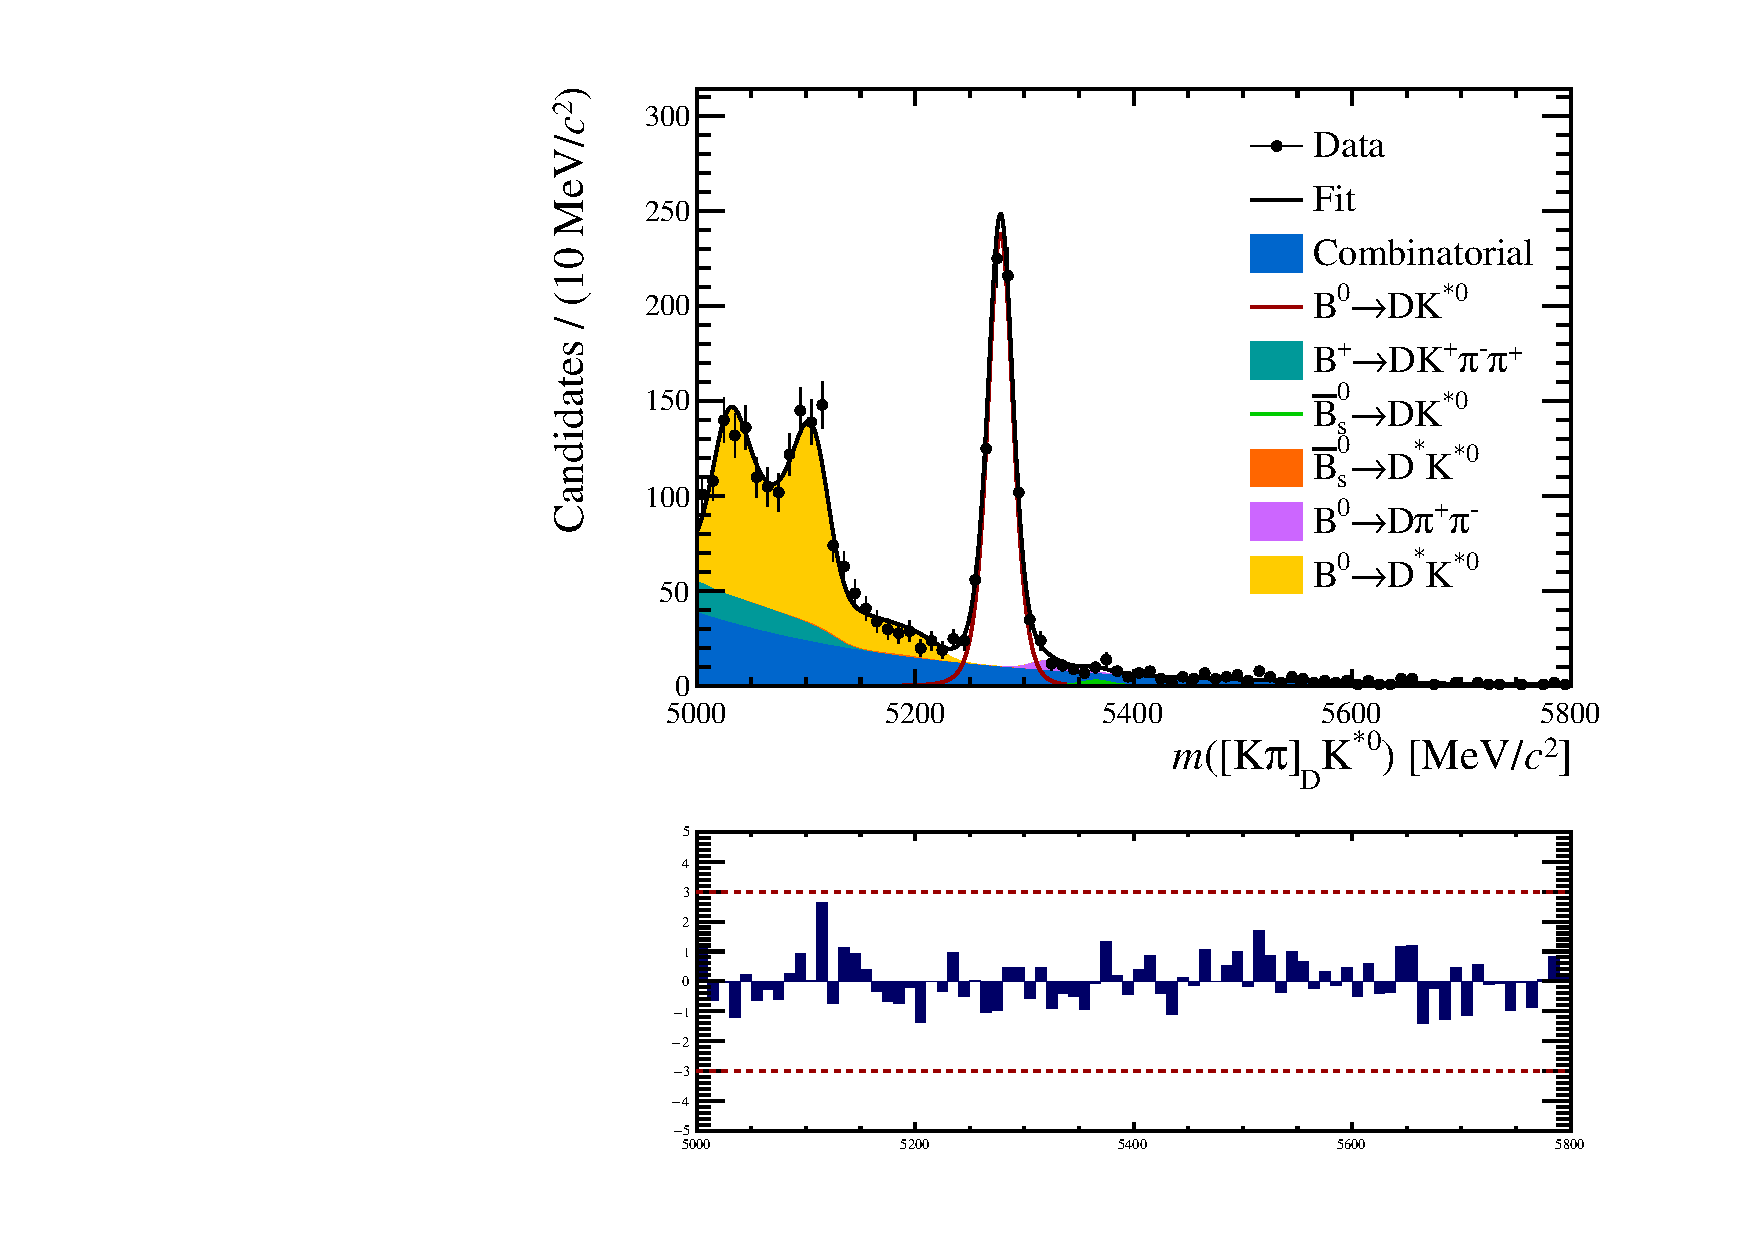
\includegraphics[width=0.5\textwidth]{ANA_resources/Plots/Data_fit/twoAndFourBody_data_split_combinedRuns_Kpi_plus.pdf}} &
        \subfloat[][$\bar{B}^0 \to D(K\pi)\bar{K}^{*0}$]{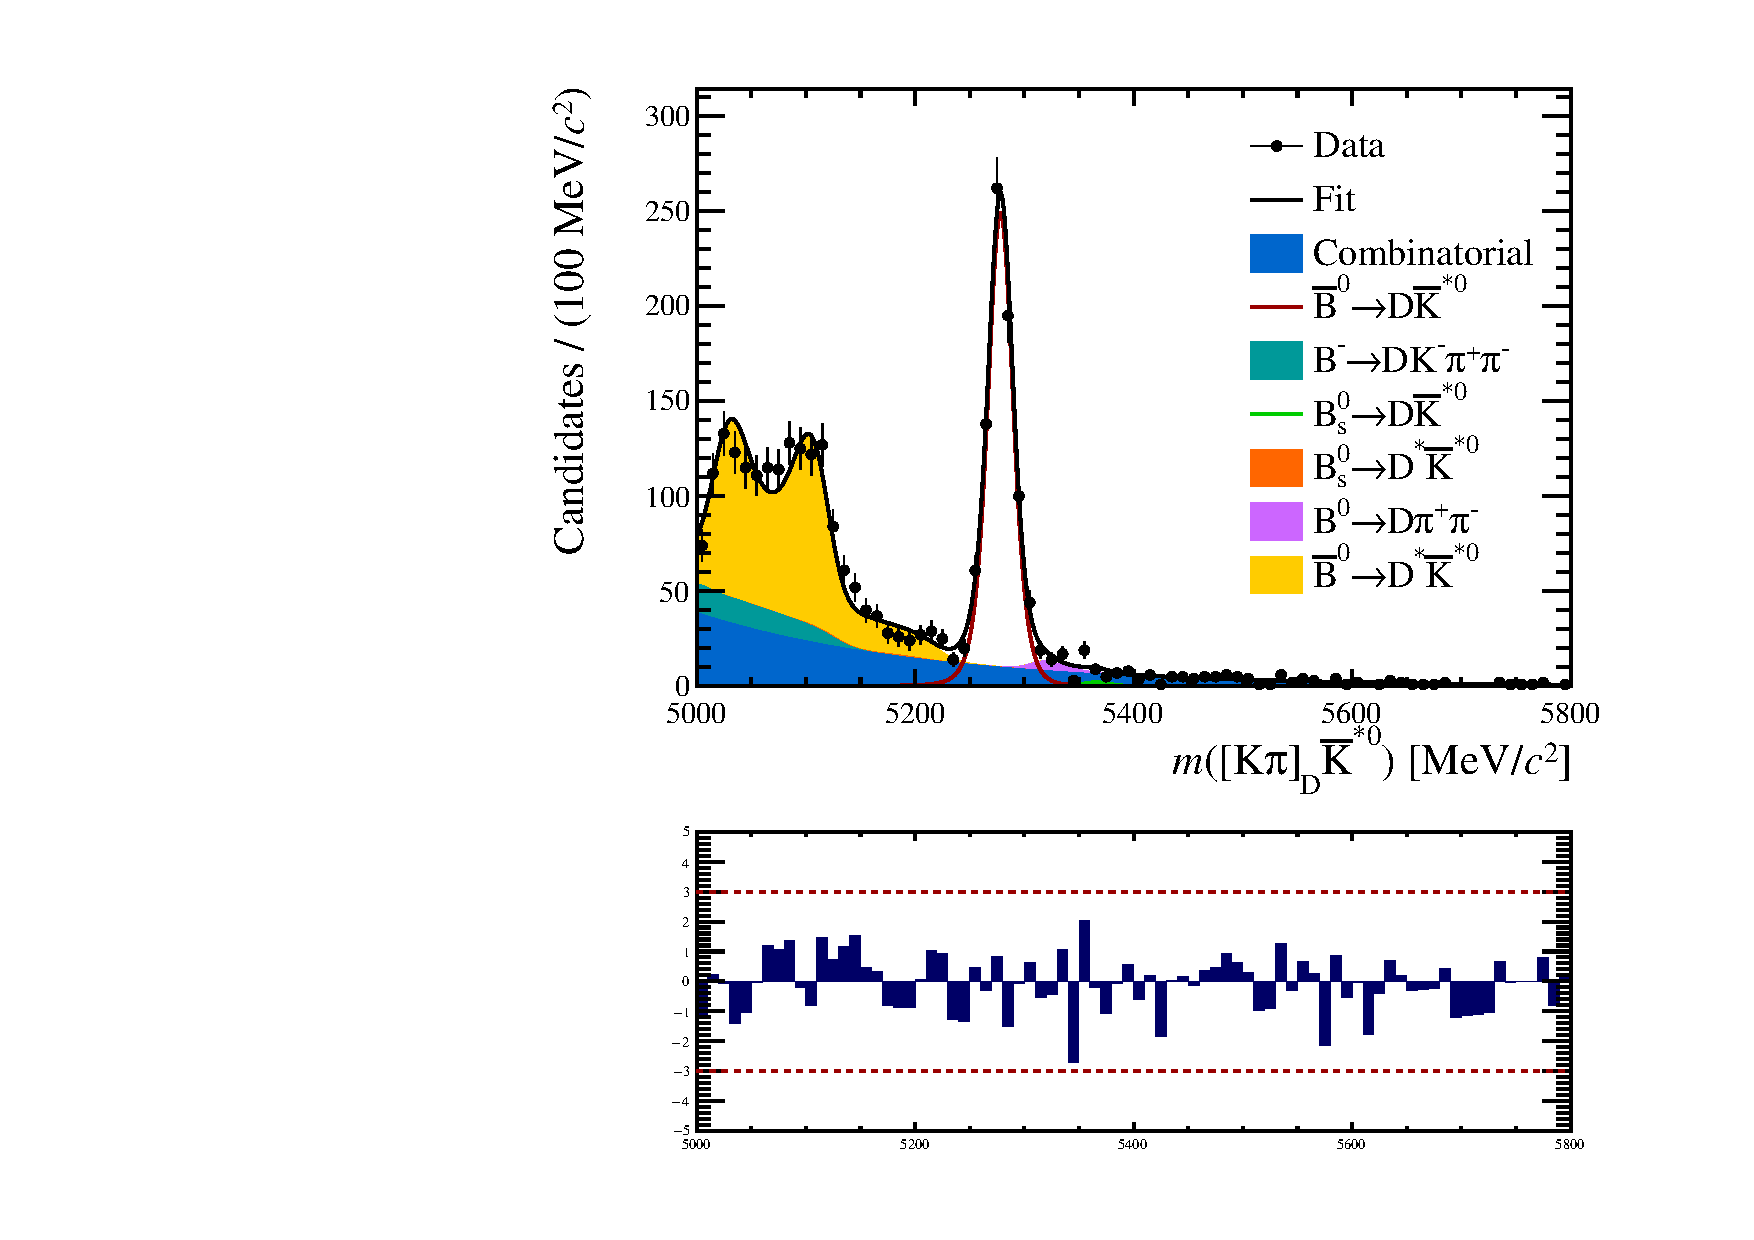
\includegraphics[width=0.5\textwidth]{ANA_resources/Plots/Data_fit/twoAndFourBody_data_split_combinedRuns_Kpi_minus.pdf}} \\
    \end{tabular}
    \caption{Fit to $B$ invariant mass of selected candidates in the $K\pi$ final state, split by $B$ flavour.}
\label{fig:data_fit_Kpi}
\end{figure}
\begin{figure}[h]
    \centering
    \begin{tabular}{cc}
        \subfloat[][$B^0 \to D(\pi K)K^{*0}$]{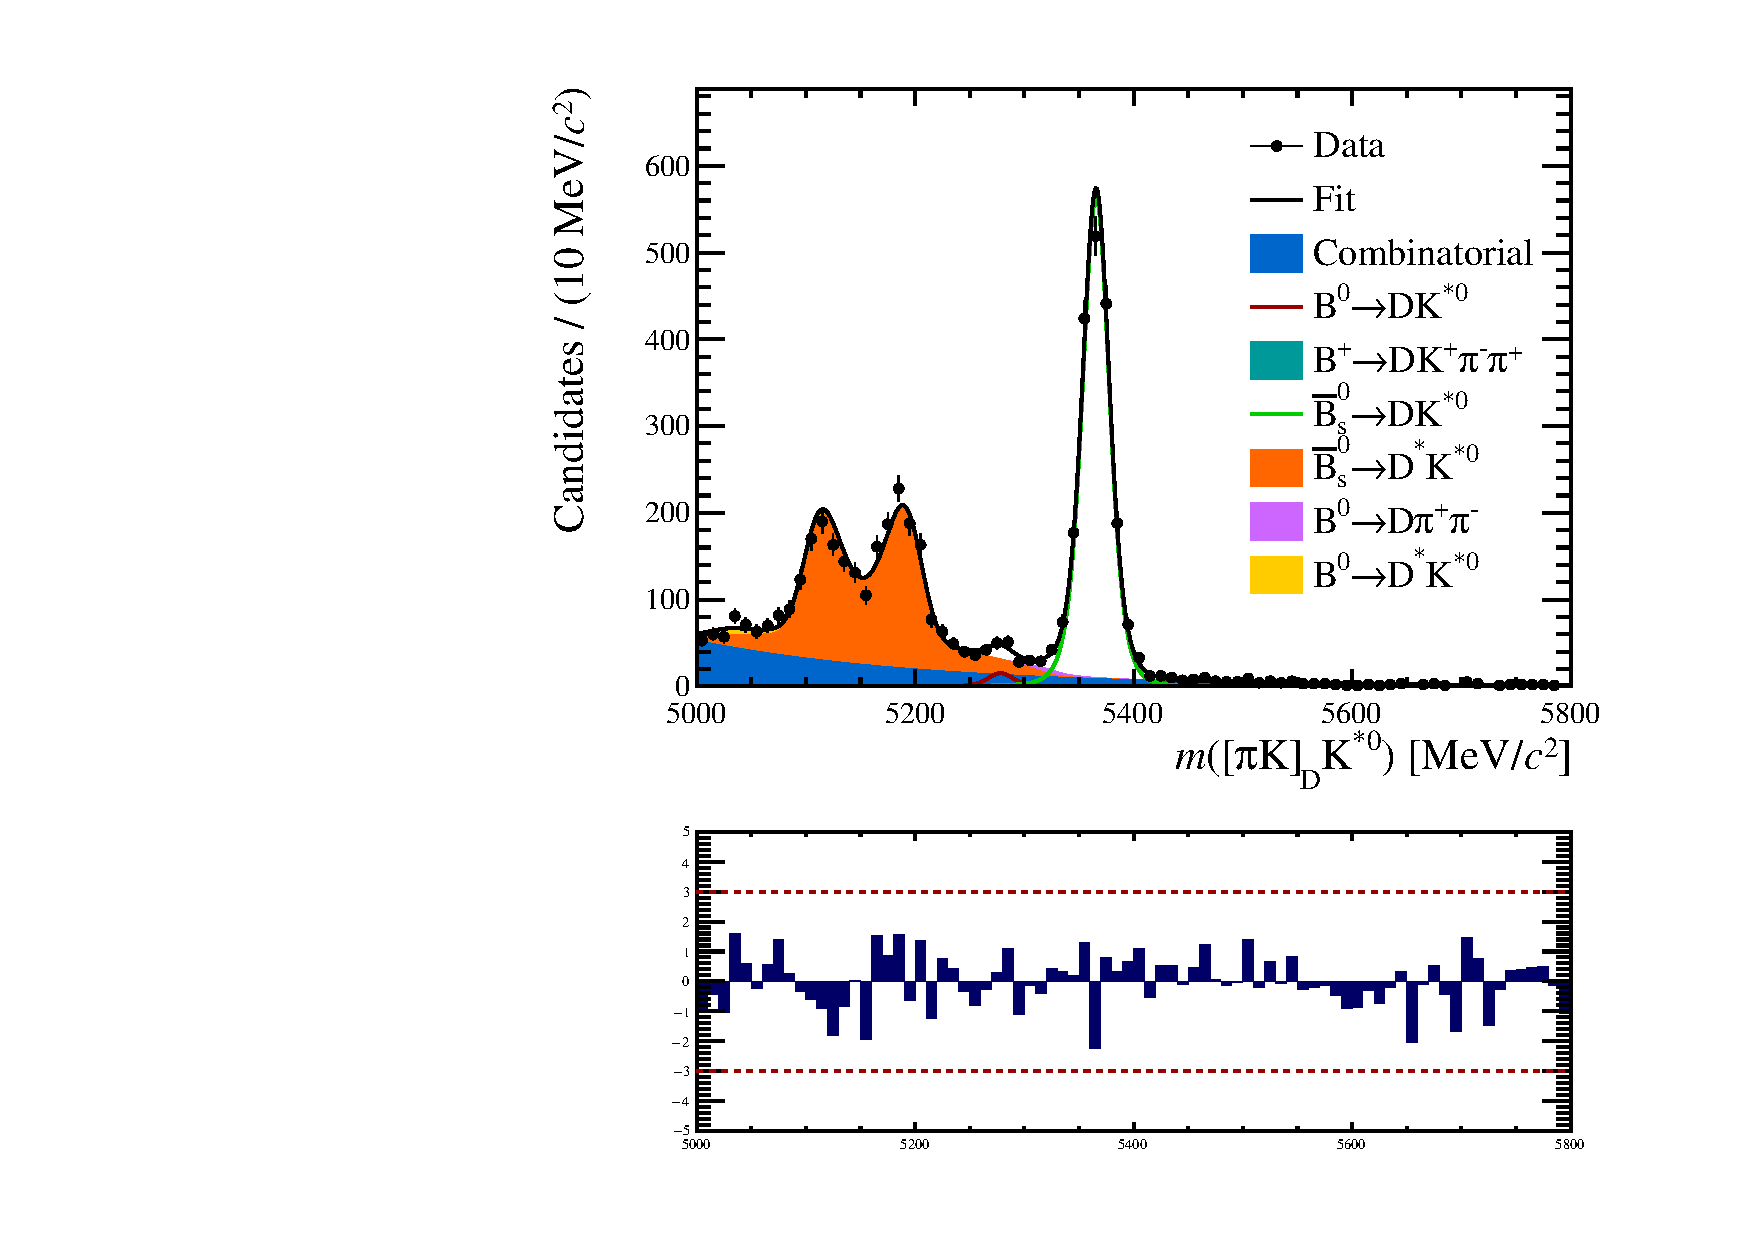
\includegraphics[width=0.5\textwidth]{ANA_resources/Plots/Data_fit/twoAndFourBody_data_split_combinedRuns_piK_plus.pdf}} &
        \subfloat[][$\bar{B}^0 \to D(\pi K)\bar{K}^{*0}$]{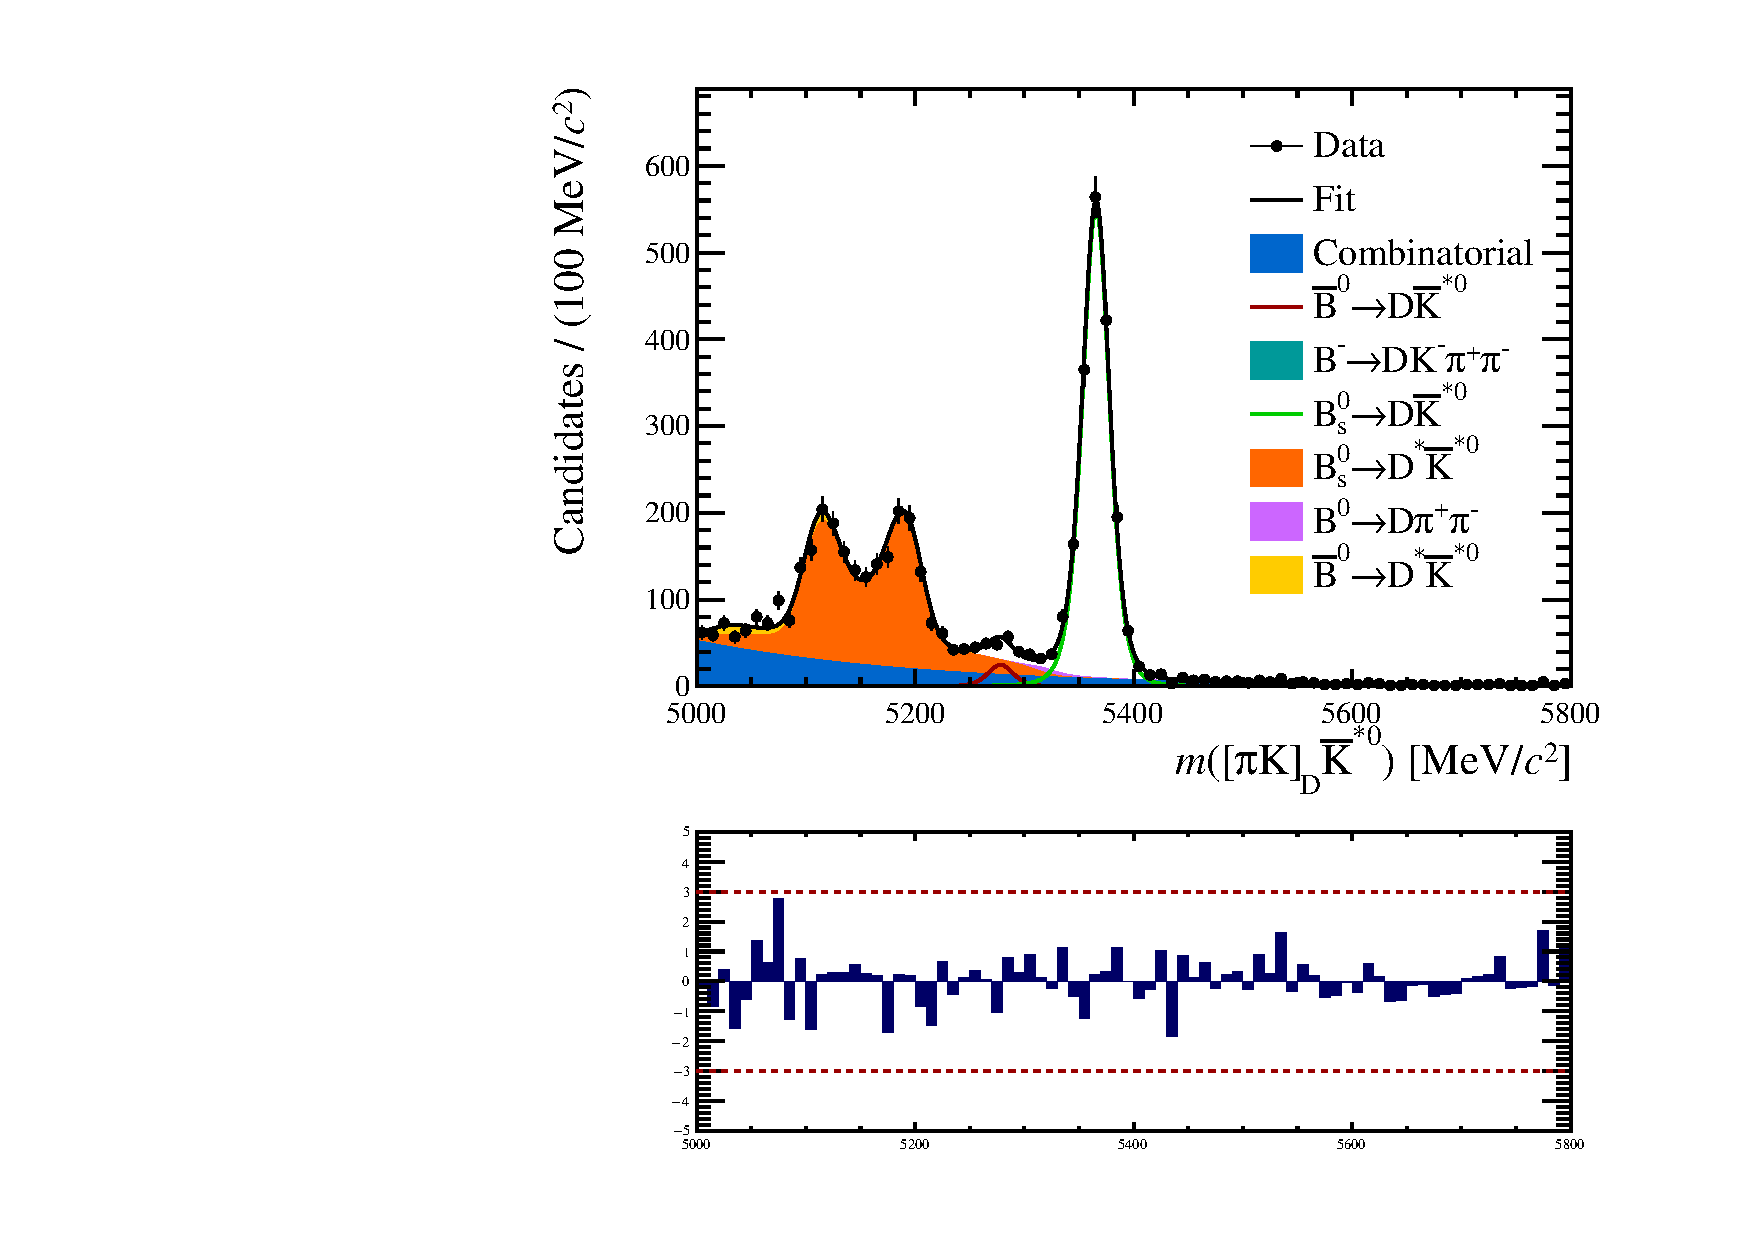
\includegraphics[width=0.5\textwidth]{ANA_resources/Plots/Data_fit/twoAndFourBody_data_split_combinedRuns_piK_minus.pdf}} \\
    \end{tabular}
    \caption{Fit to $B$ invariant mass of selected candidates in the $\pi K$ final state, split by $B$ flavour.}
\label{fig:data_fit_piK}
\end{figure}
\begin{figure}[h]
    \centering
    \begin{tabular}{cc}
        \subfloat[][$B^0 \to D(KK)K^{*0}$]{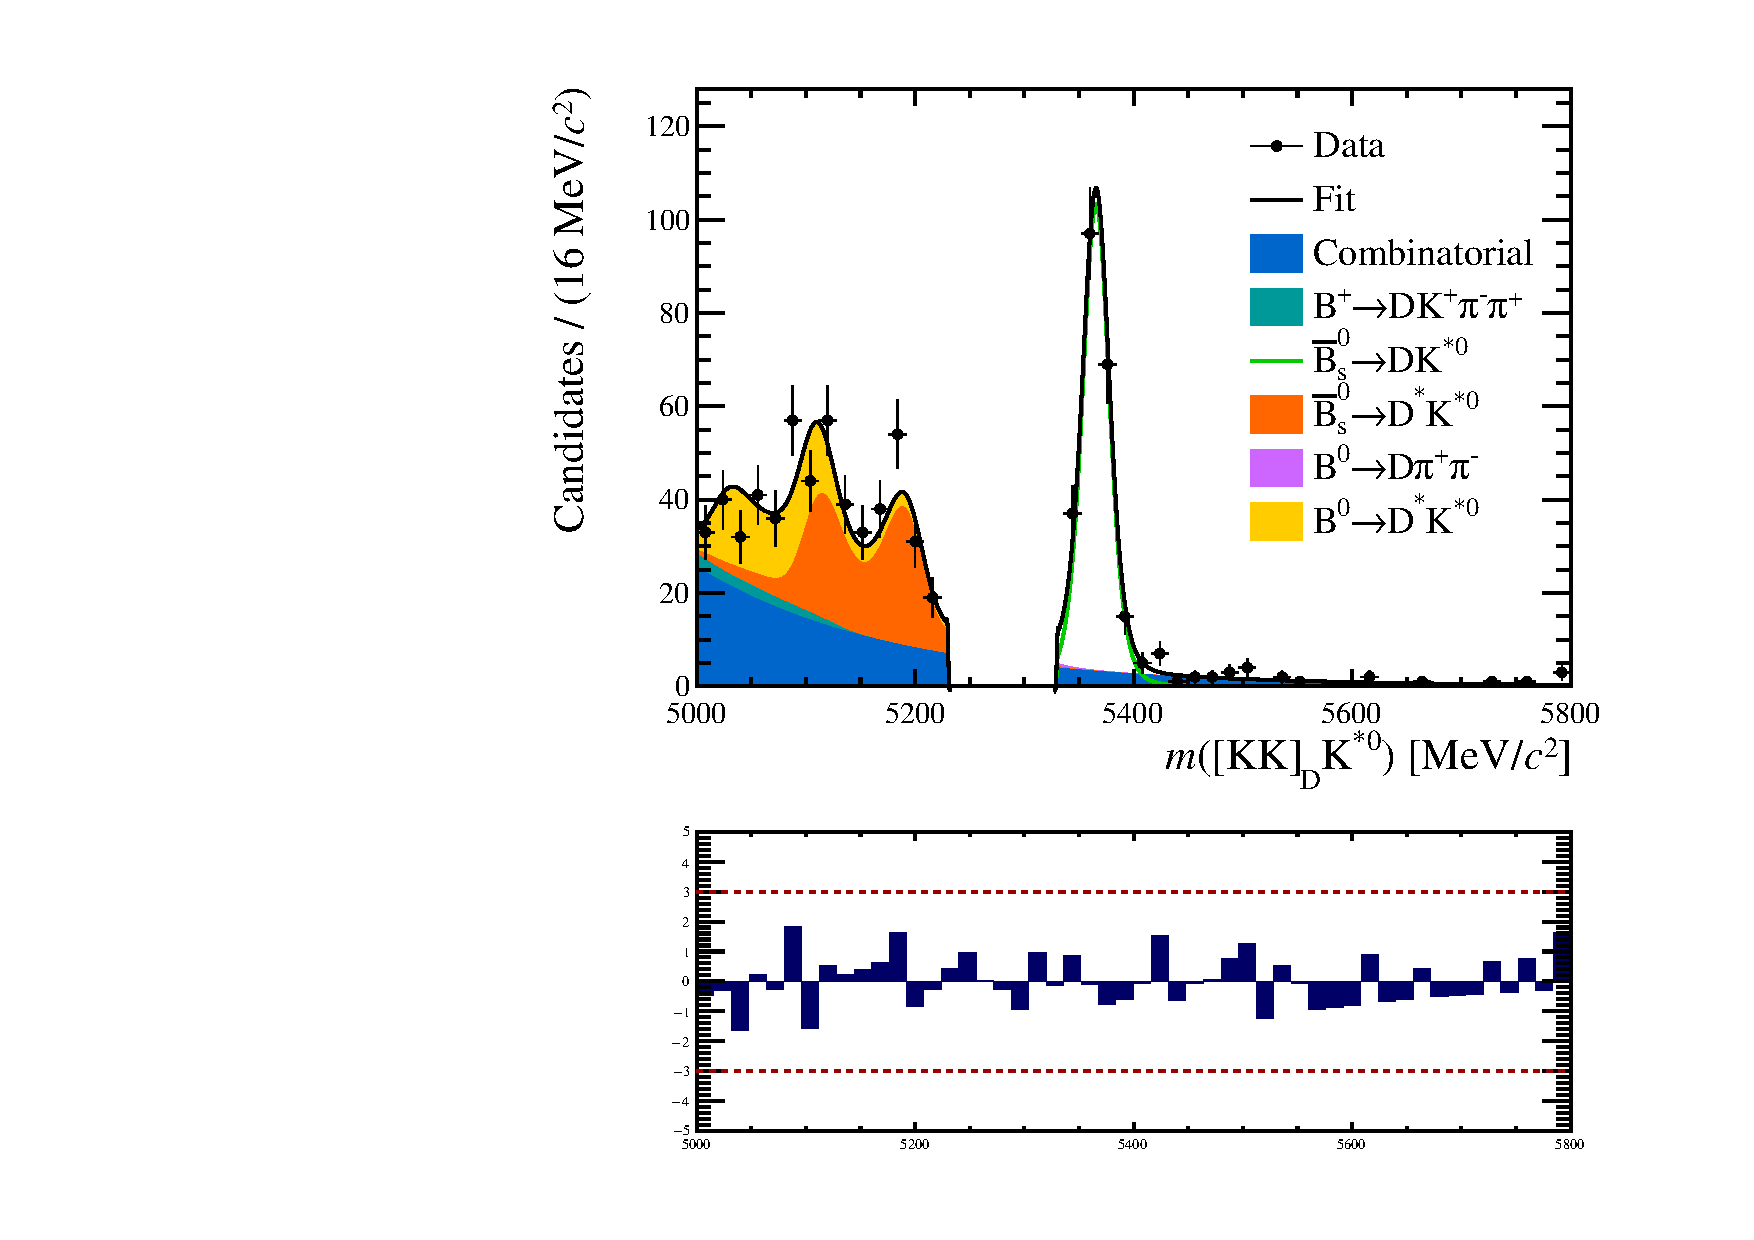
\includegraphics[width=0.5\textwidth]{ANA_resources/Plots/Data_fit/twoAndFourBody_data_split_combinedRuns_KK_plus.pdf}} &
        \subfloat[][$\bar{B}^0 \to D(KK)\bar{K}^{*0}$]{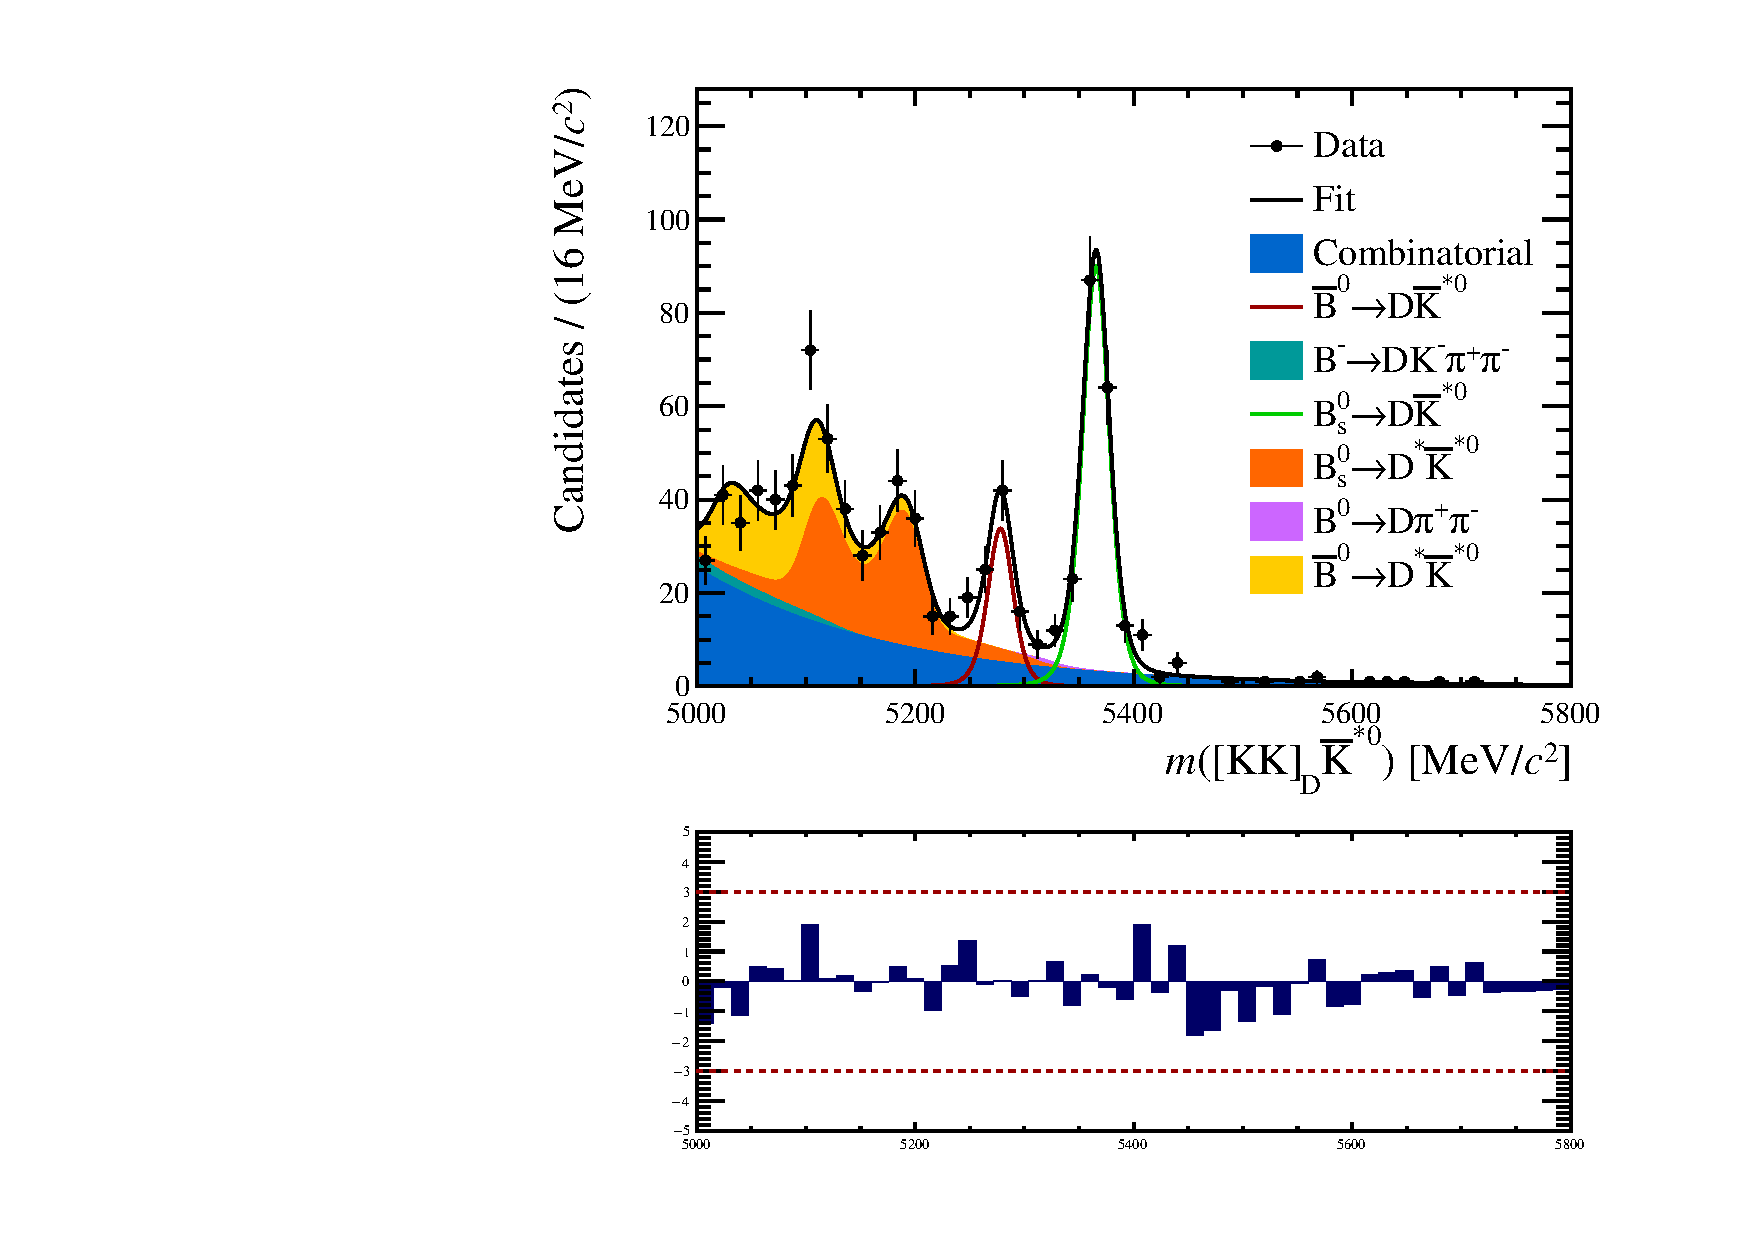
\includegraphics[width=0.5\textwidth]{ANA_resources/Plots/Data_fit/twoAndFourBody_data_split_combinedRuns_KK_minus.pdf}} \\
    \end{tabular}
    \caption{Fit to $B$ invariant mass of selected candidates in the $KK$ final state, split by $B$ flavour.}
\label{fig:data_fit_KK}
\end{figure}
\begin{figure}[h]
    \centering
    \begin{tabular}{cc}
        \subfloat[][$B^0 \to D(\pi\pi)K^{*0}$]{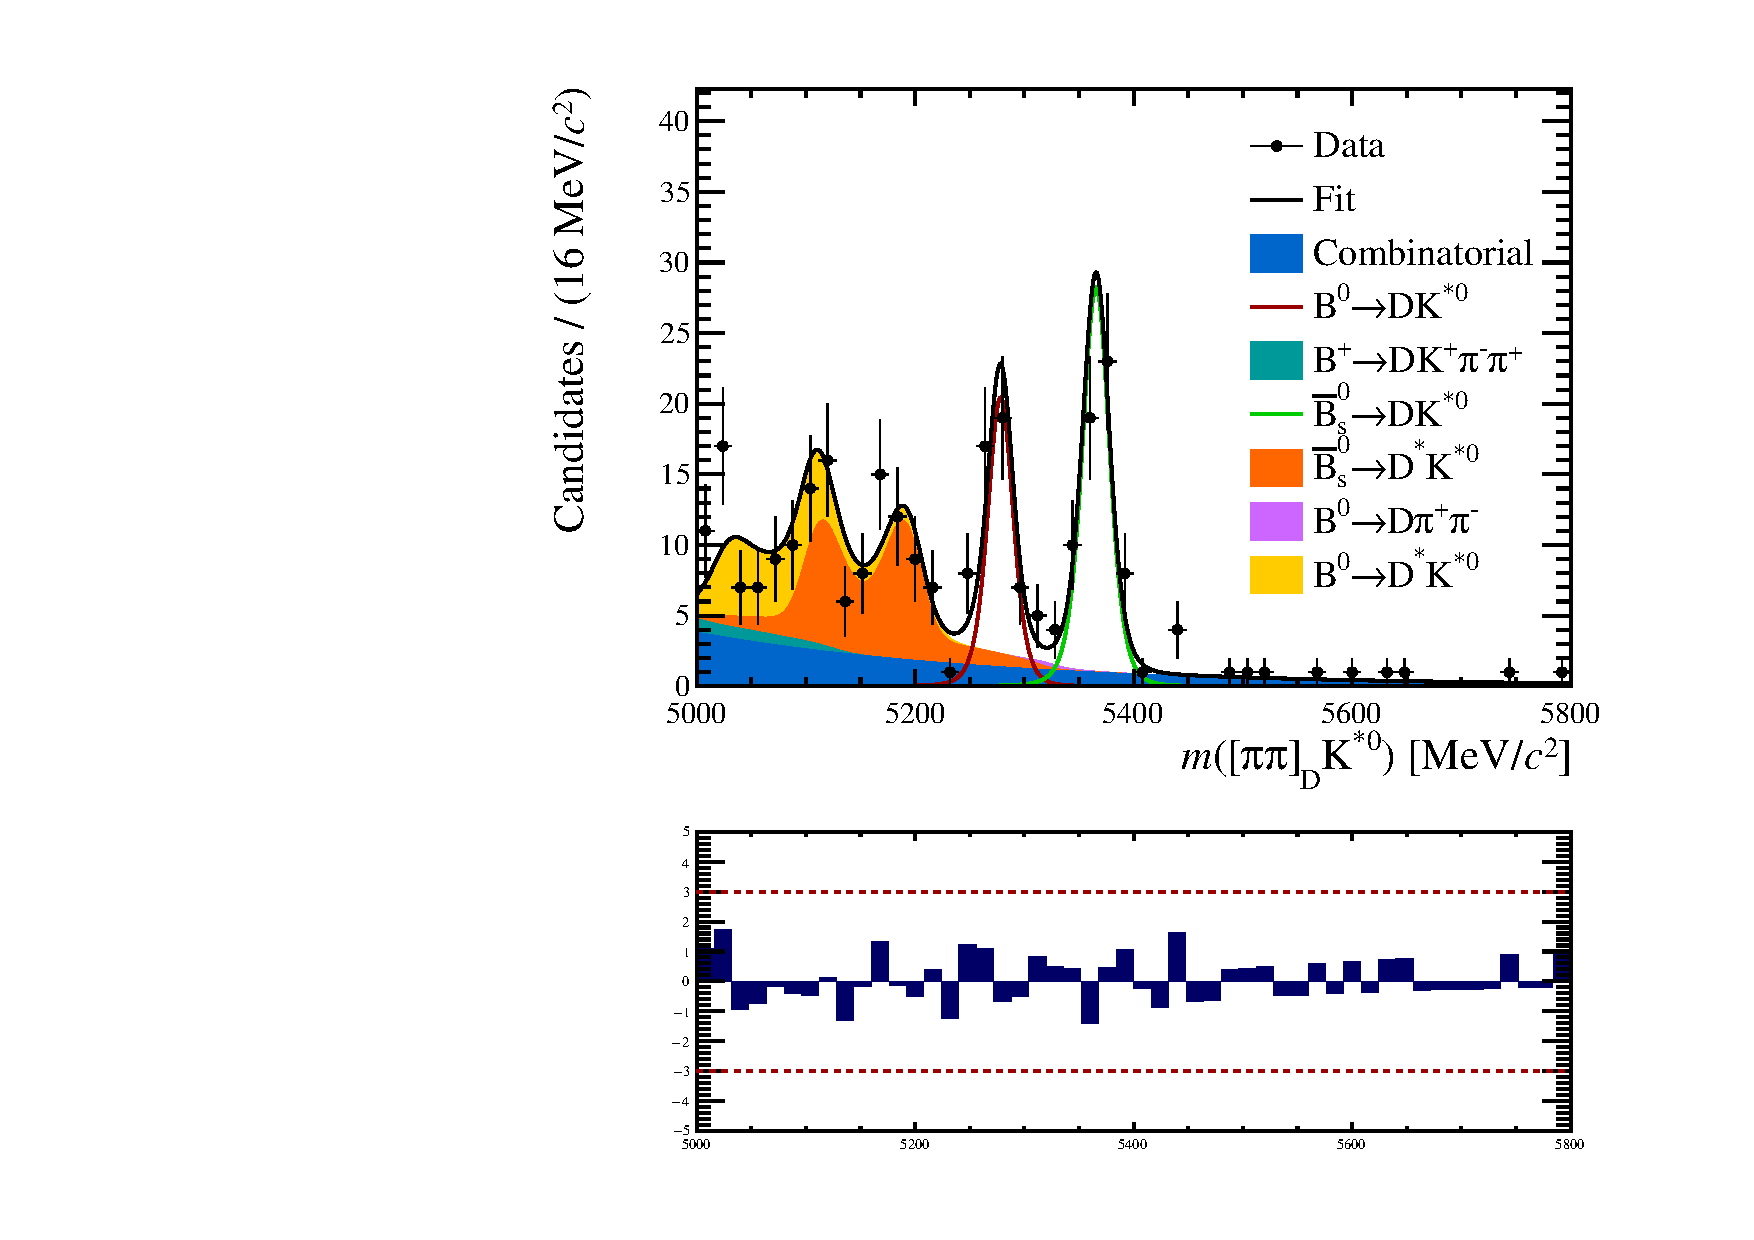
\includegraphics[width=0.5\textwidth]{ANA_resources/Plots/Data_fit/twoAndFourBody_data_split_combinedRuns_pipi_plus.pdf}} &
        \subfloat[][$\bar{B}^0 \to D(\pi\pi)\bar{K}^{*0}$]{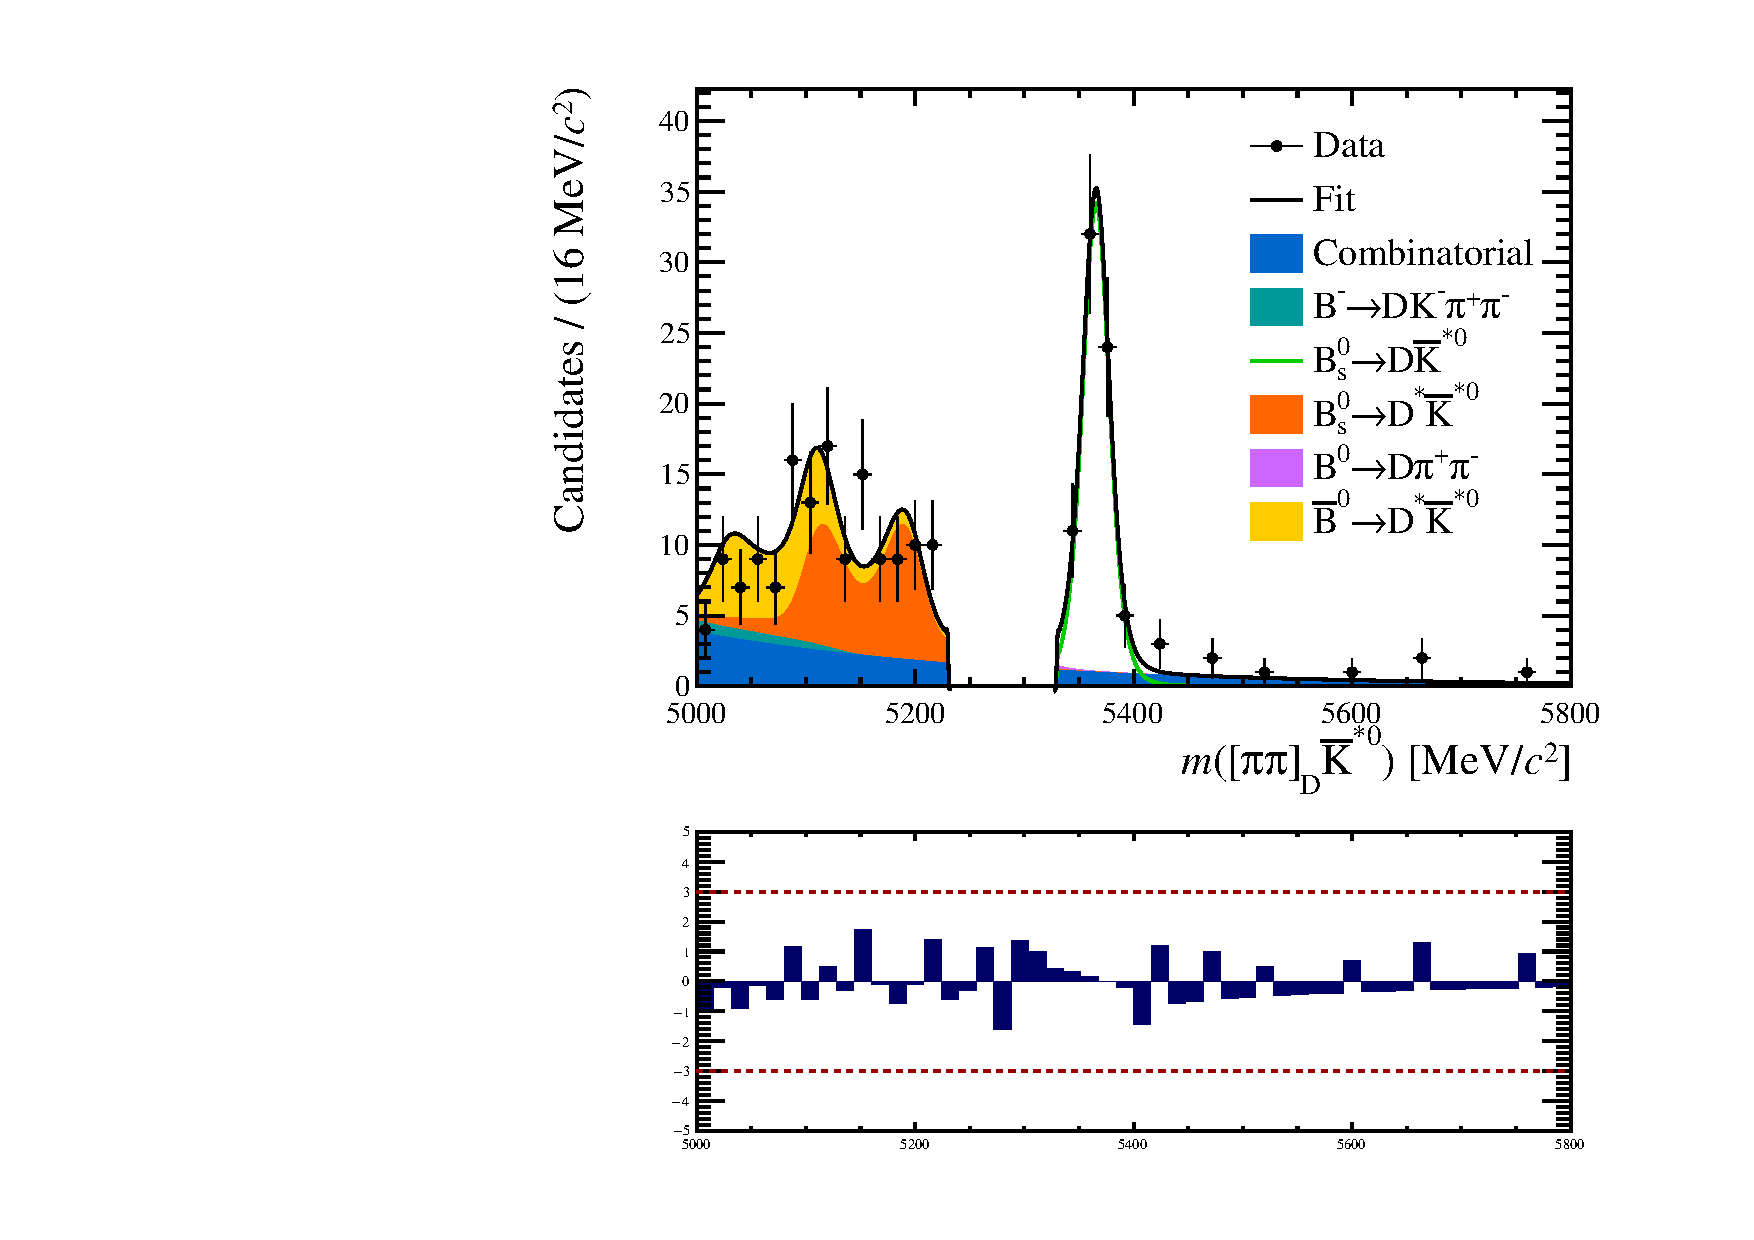
\includegraphics[width=0.5\textwidth]{ANA_resources/Plots/Data_fit/twoAndFourBody_data_split_combinedRuns_pipi_minus.pdf}} \\
    \end{tabular}
    \caption{Fit to $B$ invariant mass of selected candidates in the $\pi\pi$ final state, split by $B$ flavour.}
\label{fig:data_fit_pipi}
\end{figure}
\begin{figure}[h]
    \centering
    \begin{tabular}{cc}
        \subfloat[][$B^0 \to D(K\pi\pi\pi)K^{*0}$]{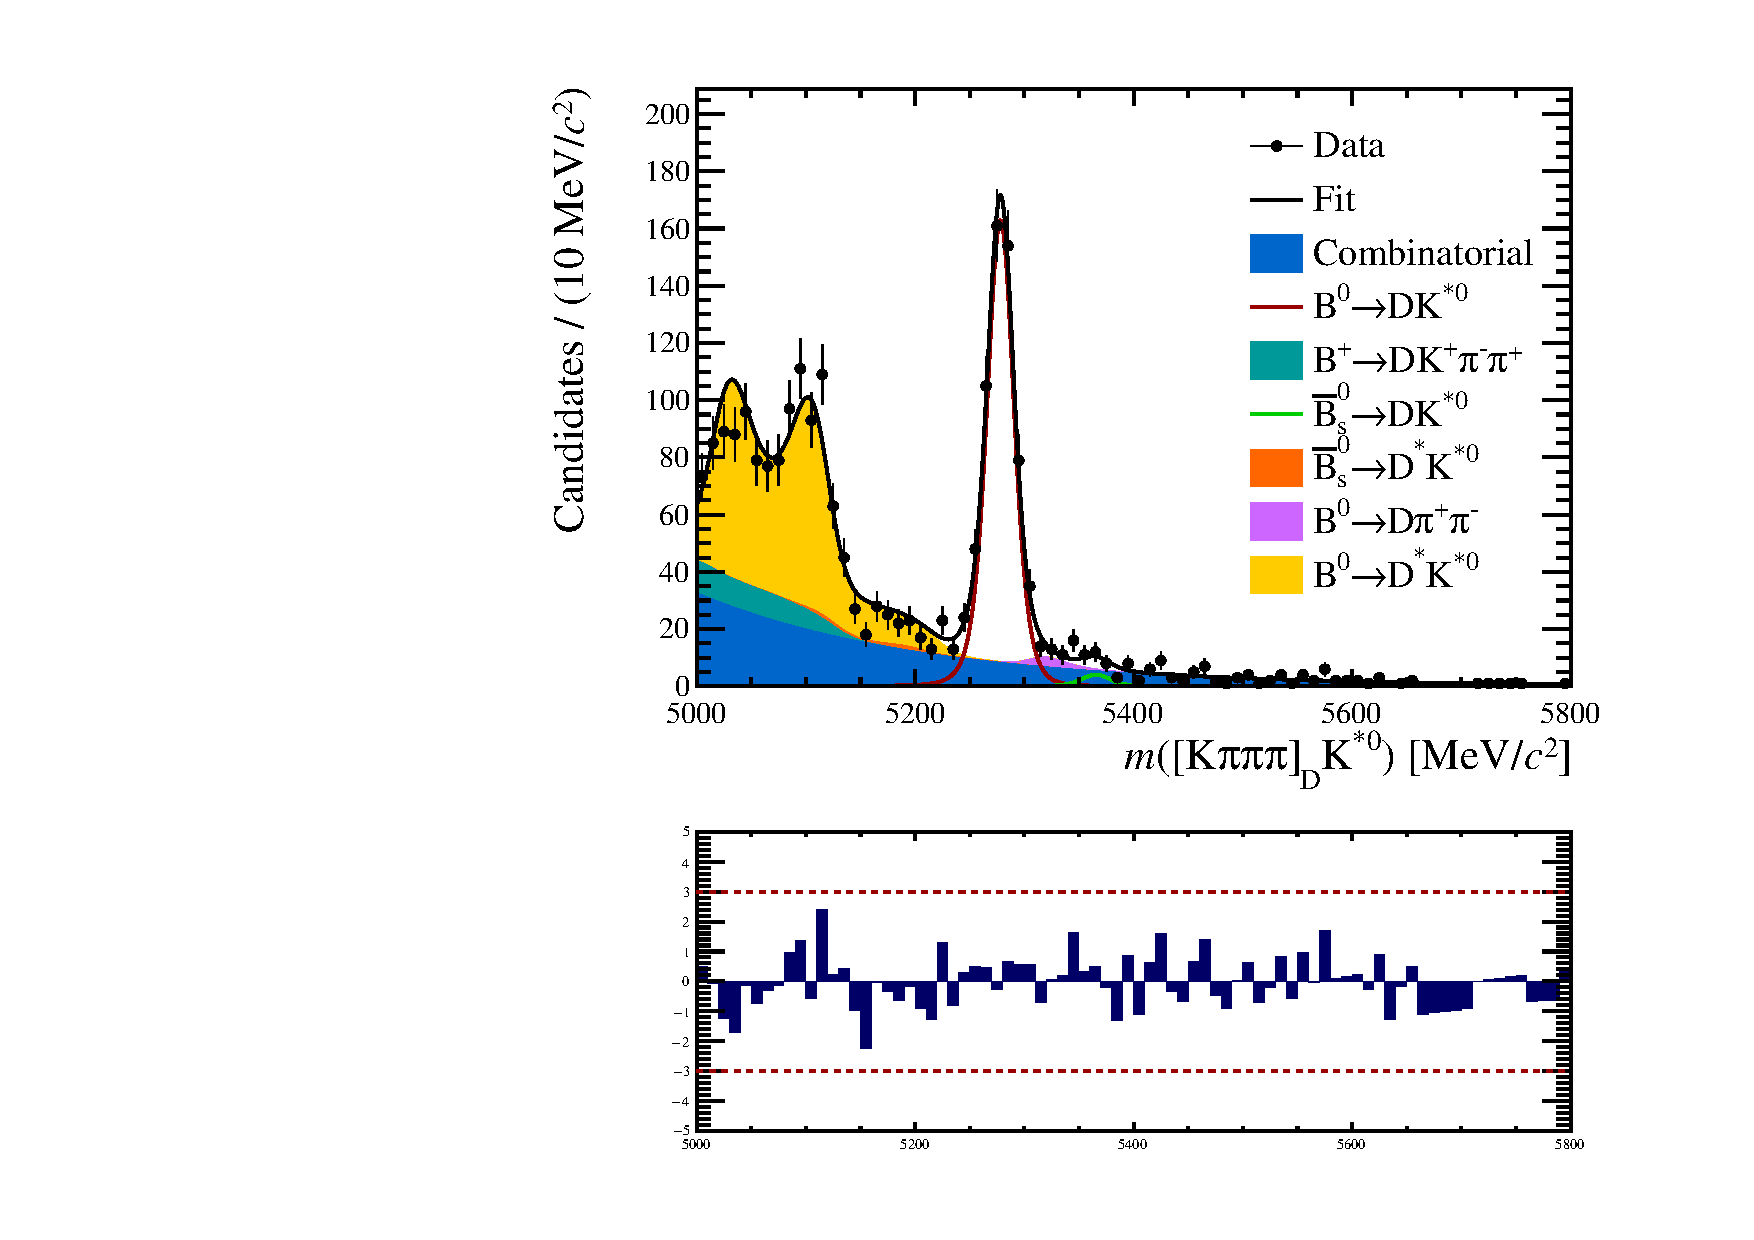
\includegraphics[width=0.5\textwidth]{ANA_resources/Plots/Data_fit/twoAndFourBody_data_split_combinedRuns_Kpipipi_plus.pdf}} &
        \subfloat[][$\bar{B}^0 \to D(K\pi\pi\pi)\bar{K}^{*0}$]{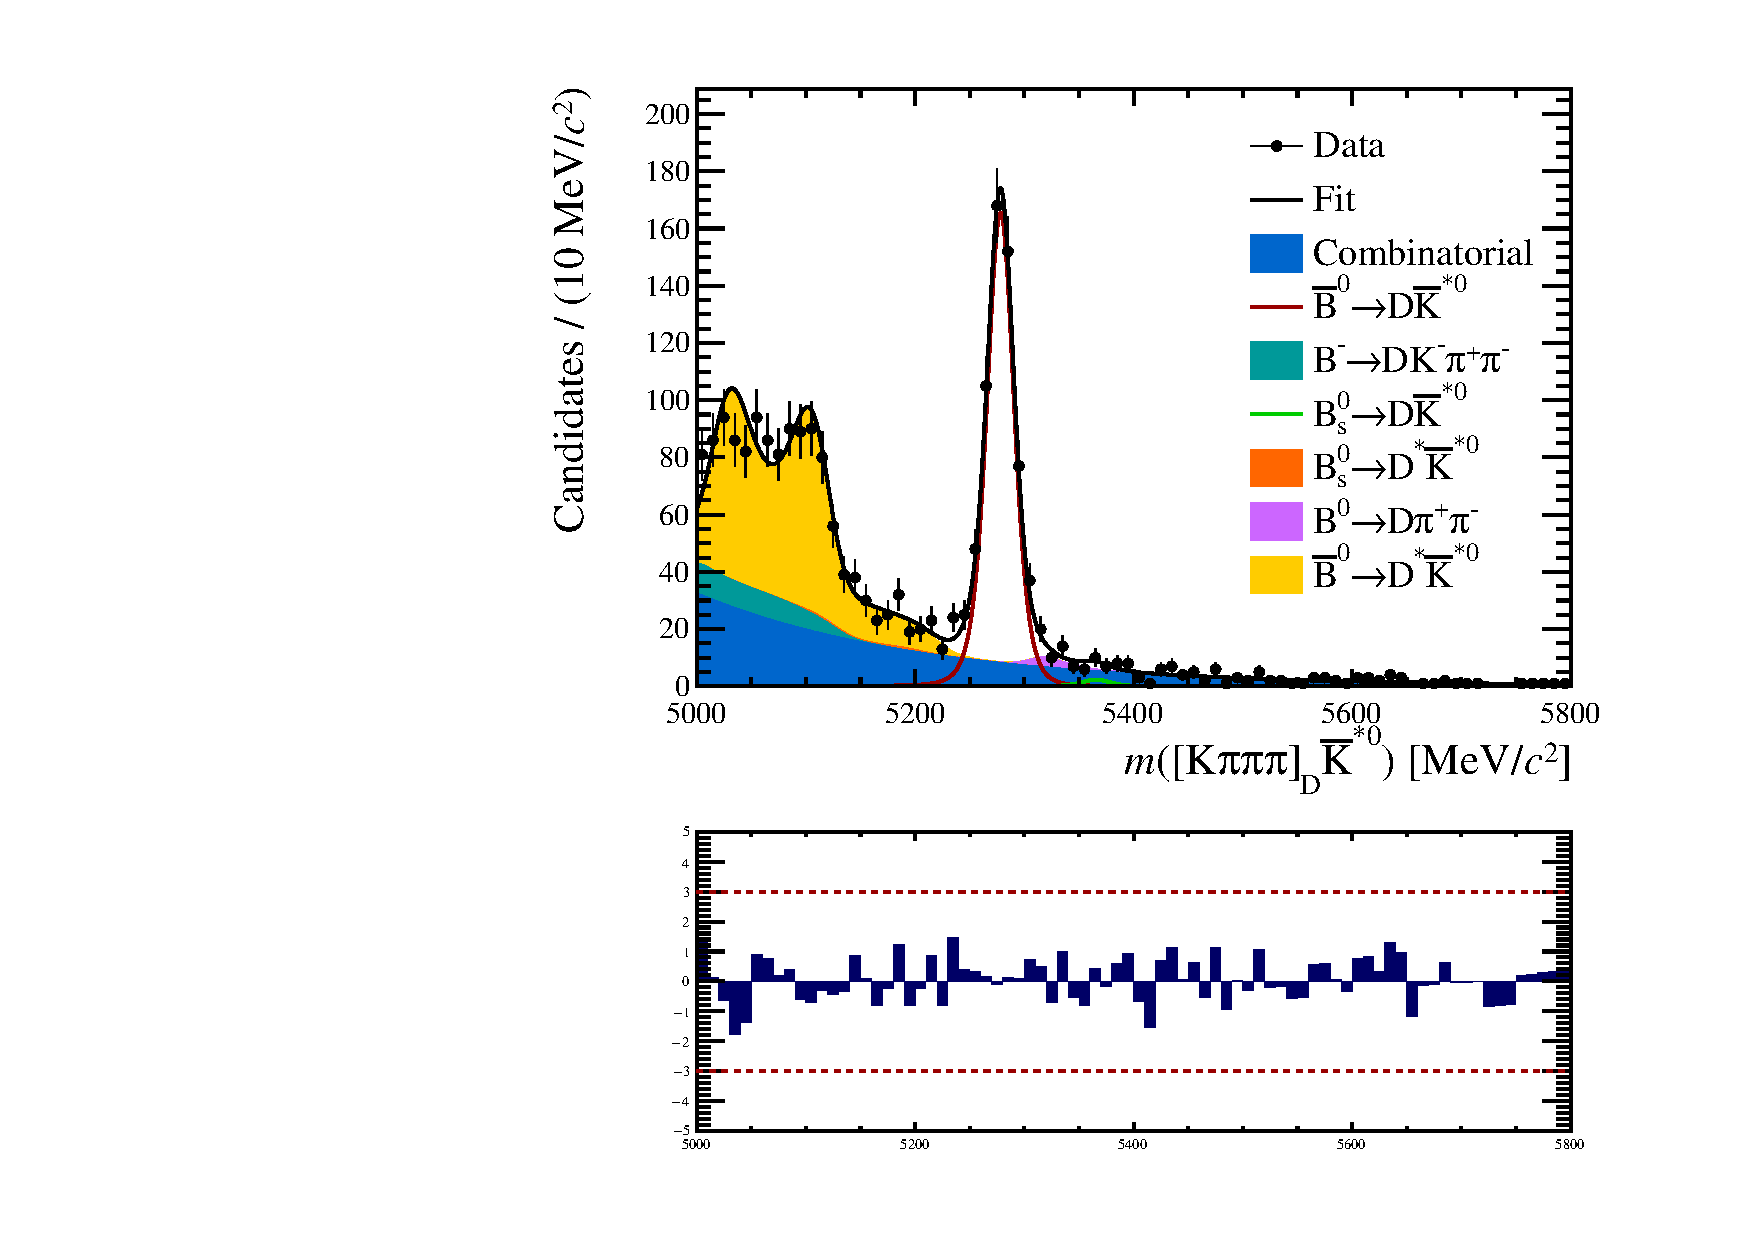
\includegraphics[width=0.5\textwidth]{ANA_resources/Plots/Data_fit/twoAndFourBody_data_split_combinedRuns_Kpipipi_minus.pdf}} \\
    \end{tabular}
    \caption{Fit to $B$ invariant mass of selected candidates in the $K\pi\pi\pi$ final state, split by $B$ flavour.}
\label{fig:data_fit_Kpipipi}
\end{figure}
\begin{figure}[h]
    \centering
    \begin{tabular}{cc}
        \subfloat[][$B^0 \to D(\pi K\pi\pi)K^{*0}$]{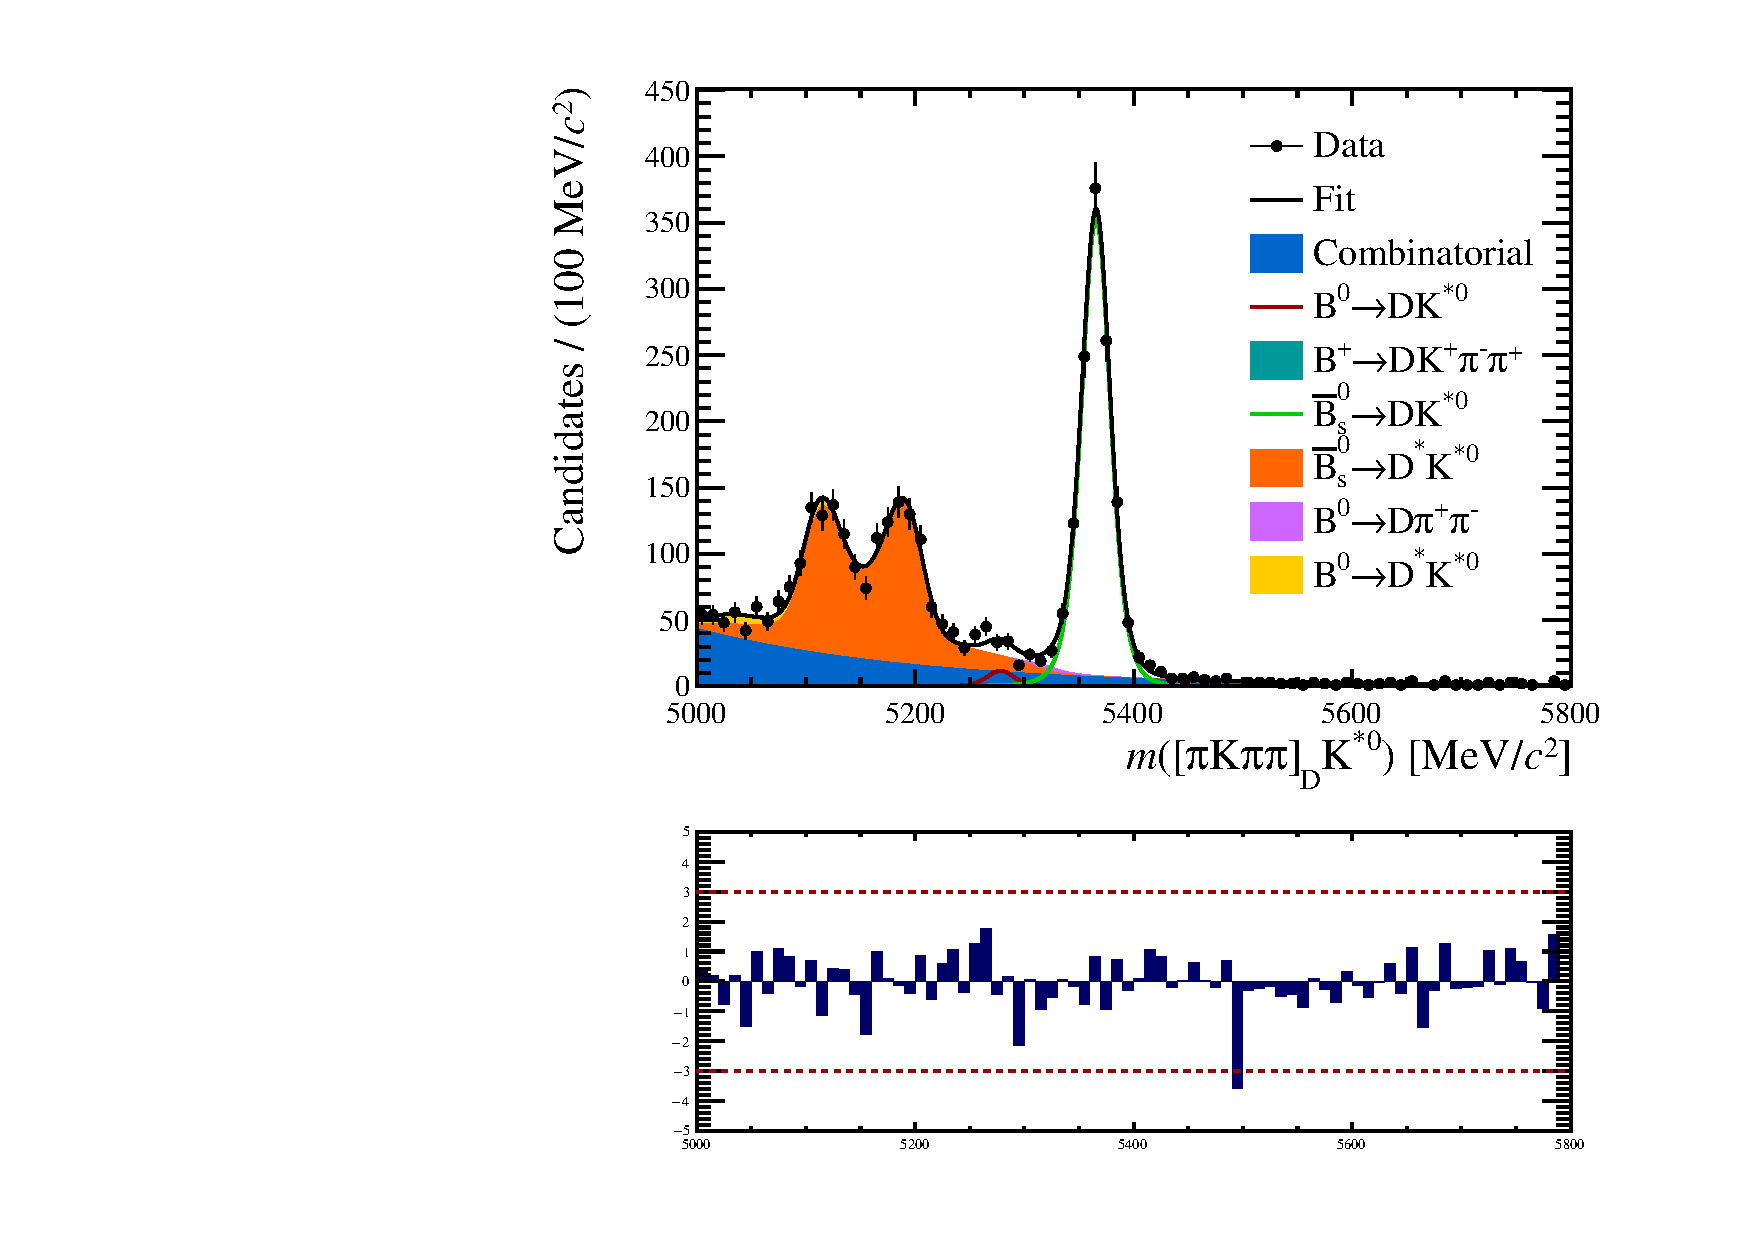
\includegraphics[width=0.5\textwidth]{ANA_resources/Plots/Data_fit/twoAndFourBody_data_split_combinedRuns_piKpipi_plus.pdf}} &
        \subfloat[][$\bar{B}^0 \to D(\pi K\pi\pi)\bar{K}^{*0}$]{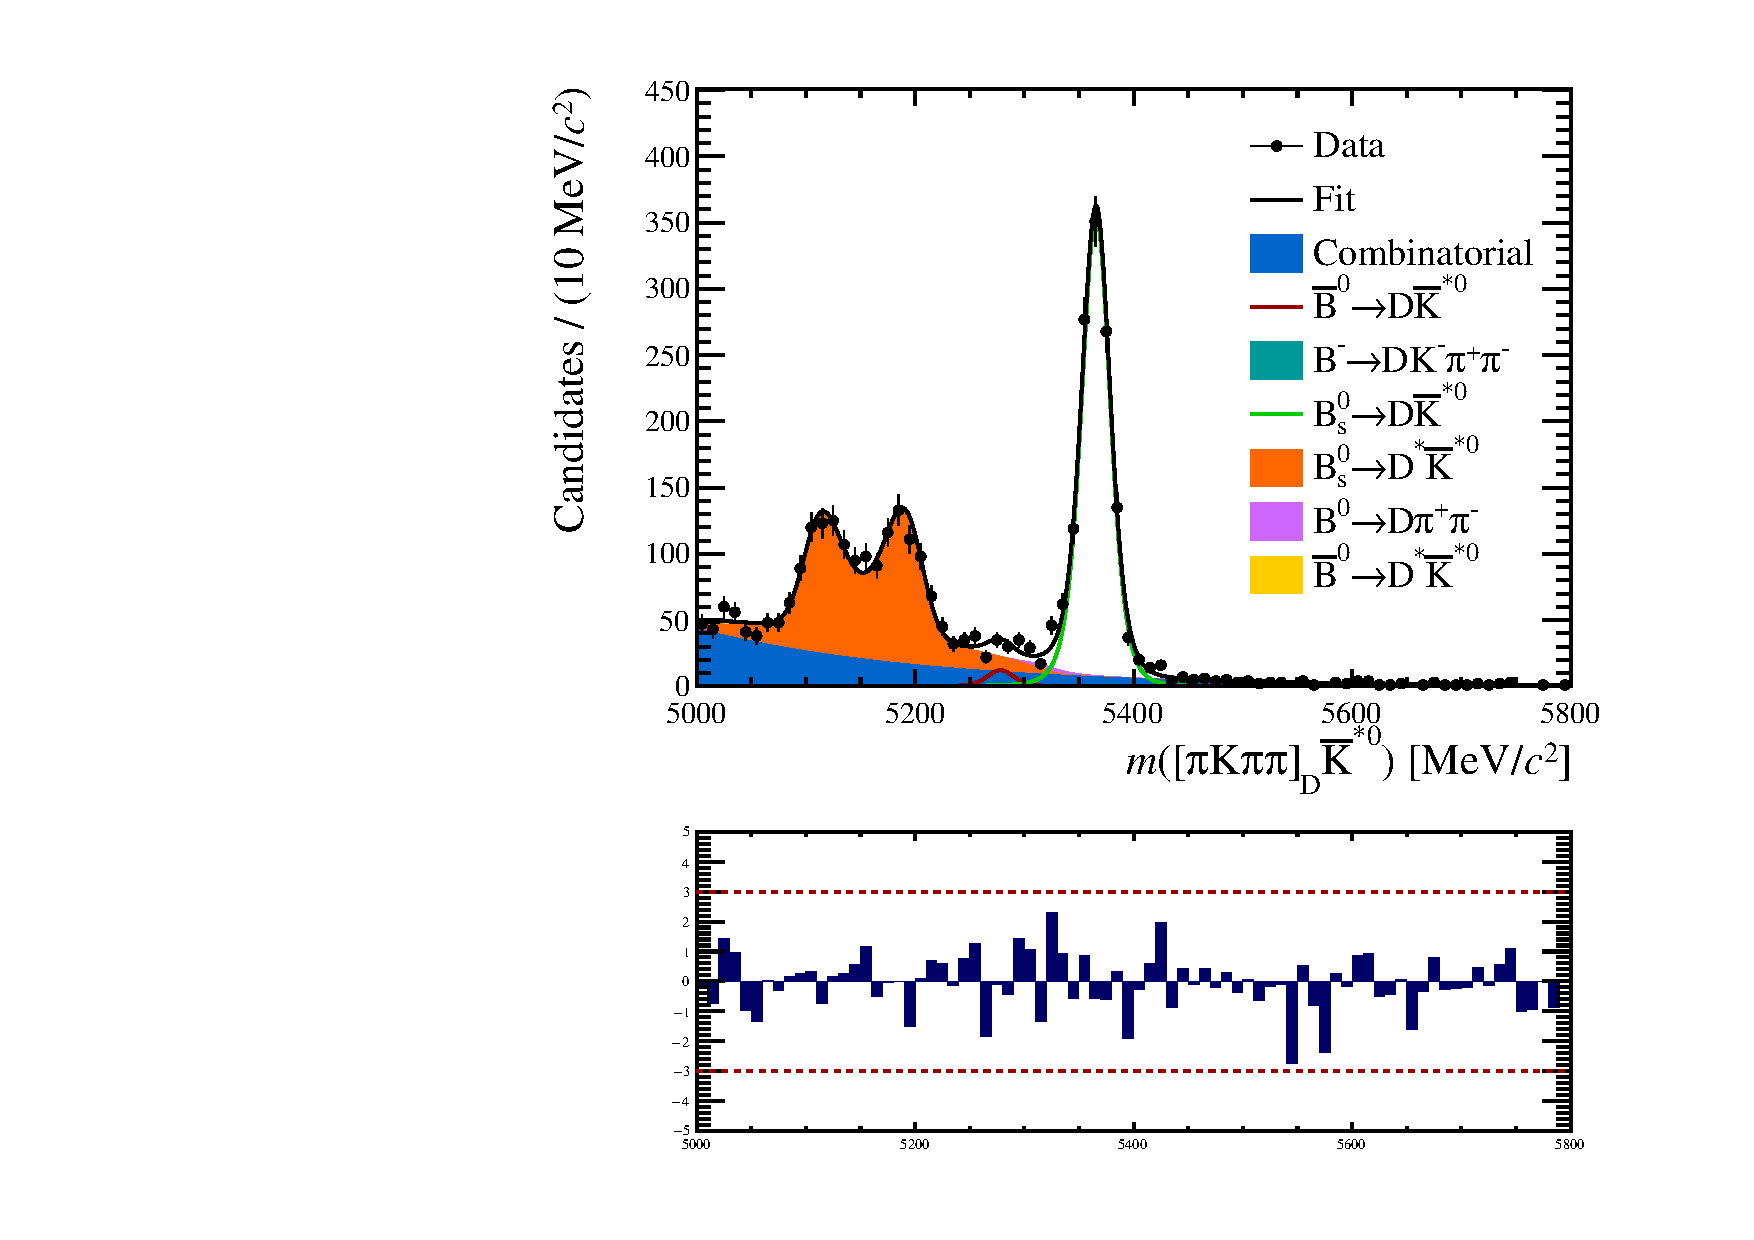
\includegraphics[width=0.5\textwidth]{ANA_resources/Plots/Data_fit/twoAndFourBody_data_split_combinedRuns_piKpipi_minus.pdf}} \\
    \end{tabular}
    \caption{Fit to $B$ invariant mass of selected candidates in the $\pi K\pi\pi$ final state, split by $B$ flavour.}
\label{fig:data_fit_piKpipi}
\end{figure}
